\chapter{Parcimonie, problèmes inverses et acquisition comprimée}
\label{chap-sparsity}
\chapteroverview{Comment décrire un signal complexe à partir d'un petit nombre de mesures ? Les représentations parcimonieuses relient la compression à la reconstruction de données incomplètes ou bruitées. Ce chapitre développe ce lien, explique le rôle de l'optimisation convexe et précise les hypothèses qui permettent de garantir une reconstruction par acquisition comprimée.}

\section{Du signal continu aux échantillons}
\label{sec-sampling}
Un dispositif d'acquisition transforme un signal continu $\tilde f$ en un vecteur fini $f=(f_q)_{q=1}^Q\in\RR^Q$. Pour un son, ces valeurs correspondent à des mesures effectuées à des instants successifs. Pour une image en niveaux de gris, elles représentent la lumière reçue par de petites surfaces du capteur. Une mesure de pixel idéalisée s'écrit
\[
 f_q=\int_{c_q}\tilde f(s)\,\d s,
\]
où $c_q$ est la surface de l'élément sensible. Diviser par son aire donne une intensité moyenne ; le temps d'exposition et l'étalonnage introduisent d'autres facteurs d'échelle. Les signaux en couleur ou multicanaux se décrivent en enregistrant plusieurs valeurs à chaque position.

\begin{figure}[htbp]\centering
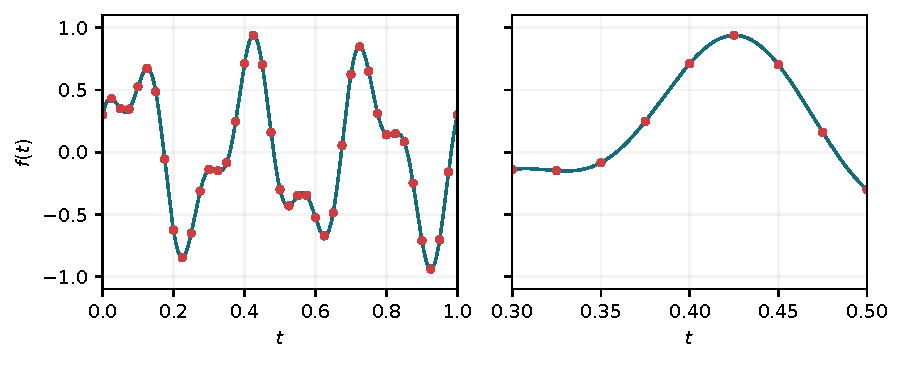
\includegraphics[width=.48\linewidth]{chapter-sampling/discrete-signal.pdf}\hfill
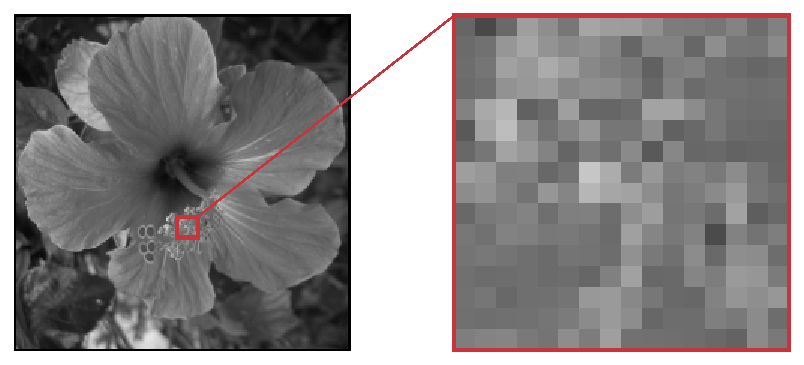
\includegraphics[width=.48\linewidth]{chapter-sampling/discrete-image.pdf}
\caption{Échantillonnage d'un signal unidimensionnel et d'une image. Les points indiquent les échantillons temporels ; les cadres rouges repèrent la région de l'image agrandie à droite.}\label{fig-samples}
\end{figure}

L'échantillonnage préserve l'information sous des hypothèses appropriées. Supposons par exemple que $\tilde f\in L^2(\RR)$ ait une transformée de Fourier à support dans $[-B,B]$, la fréquence étant mesurée en cycles par unité de temps. Si le pas vérifie $0<T<1/(2B)$, le théorème d'échantillonnage~\cite{shannon1949} donne
\[
 \tilde f(t)=\sum_{k\in\ZZ}\tilde f(kT)\,
 \operatorname{sinc}\!\left(\frac{t}{T}-k\right),
 \qquad \operatorname{sinc}(u)=\begin{cases}\sin(\pi u)/(\pi u),&u\ne0,\\1,&u=0.\end{cases}
\]
Pour le représentant continu de cette fonction à bande limitée, la série converge dans $L^2$ et uniformément. Le théorème utilise les échantillons sur tout l'axe temporel. Un enregistrement fini, la quantification et le bruit de mesure introduisent des erreurs supplémentaires. Les fréquences dépassant la bande d'acquisition doivent être atténuées avant l'échantillonnage pour éviter le repliement spectral ; augmenter ensuite la précision numérique ne supprime pas ce repliement.

L'échantillonnage concerne la représentation d'un signal continu par des mesures, tandis que le codage sans perte concerne la représentation binaire de ces mesures. La parcimonie fournit une autre hypothèse utile sur le signal et conduit à une autre stratégie d'acquisition.

\Needspace{6\baselineskip}
\section{Approximation non linéaire et compression}
\subsection{Représentations parcimonieuses}
Un dictionnaire $\Psi=(\psi_n)_{n=1}^N$ est une famille de vecteurs $\psi_n\in\RR^Q$. On cherche une approximation
\[
 f\approx\Psi x=\sum_{n=1}^N x_n\psi_n
\]
comportant peu de coefficients non nuls. Les sinusoïdes, les cosinus locaux et les ondelettes sont des exemples d'atomes. Le codage par transformée utilise ces représentations pour concentrer une grande partie de l'énergie du signal dans un petit nombre de coefficients.

Pour un budget entier $0\le M\le N$, une meilleure approximation à $M$ termes résout
\begin{equation}\label{eq-pbm-approx}
 x^\star\in\arg\min_{x\in\RR^N,\;\norm{x}_0\le M}\norm{f-\Psi x}_2^2,
 \qquad \norm{x}_0=\#\{n:x_n\ne0\}.
\end{equation}
On note ici $\norm{v}_2^2=\sum_n|v_n|^2$. La notation $\norm{x}_0$ est conventionnelle : ce comptage n'est pas une norme, car multiplier un vecteur non nul par un scalaire non nul ne change pas le nombre de ses composantes non nulles. Pour un dictionnaire général, l'approximation parcimonieuse est un problème NP-difficile~\cite{Natarajan95}. Tester tous les supports possibles est généralement prohibitif ; cette difficulté dans le pire cas n'exclut pas des algorithmes efficaces pour certains dictionnaires ou certaines données.

\subsection{Le cas orthonormal}
Supposons $N=Q$ et $\Psi$ base orthonormale, c'est-à-dire $\langle\psi_n,\psi_m\rangle=\delta_{nm}$. En posant $a_n=\langle f,\psi_n\rangle$, l'identité de Parseval donne
\begin{equation}\label{eq-expansion-bon}
 f=\sum_{n=1}^N a_n\psi_n,
 \qquad \norm{f-\Psi x}_2^2=\sum_{n=1}^N|a_n-x_n|^2.
\end{equation}
Une fois le support choisi, les meilleurs coefficients sont les $a_n$ correspondants. Pour minimiser l'énergie éliminée, on conserve les $M$ plus grandes amplitudes. Plus précisément, choisissons un ordre $|a_{n_1}|\ge\cdots\ge|a_{n_N}|$. Alors
\begin{equation}\label{eq-formule-thresh}
 x_n^\star=\begin{cases}
 a_n,&n\in\{n_1,\ldots,n_M\},\\
 0,&\text{sinon}.
 \end{cases}
\end{equation}
Des égalités d'amplitude au niveau du seuil peuvent donner plusieurs minimiseurs. S'il y a moins de $M$ coefficients non nuls, l'approximation utilise moins de $M$ termes.

\begin{figure}[htbp]\centering
\begin{tabular}{@{}c@{\hspace{2mm}}c@{\hspace{2mm}}c@{\hspace{2mm}}c@{}}
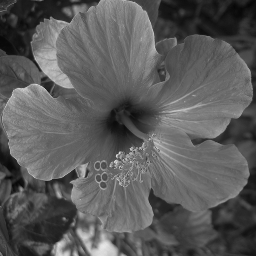
\includegraphics[width=.235\linewidth]{chapter-sampling/original.png}&
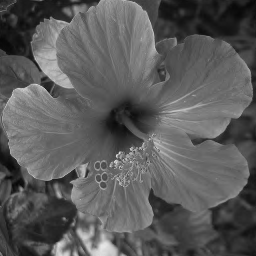
\includegraphics[width=.235\linewidth]{chapter-sampling/approx-4.png}&
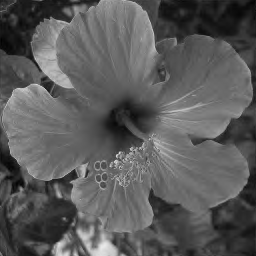
\includegraphics[width=.235\linewidth]{chapter-sampling/approx-8.png}&
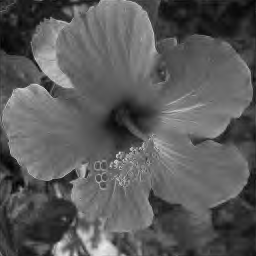
\includegraphics[width=.235\linewidth]{chapter-sampling/approx-16.png}\\
$f$&$M=N/4$&$M=N/8$&$M=N/16$
\end{tabular}
\caption{Meilleures approximations à $M$ termes d'une image de fleur de $N=256^2$ pixels. La transformée orthonormale utilise des ondelettes de Daubechies à quatre moments nuls, cinq niveaux et des conditions périodiques au bord. Les intensités affichées sont tronquées à $[0,1]$.}\label{fig-approx}
\end{figure}

La reconstruction $x\mapsto\Psi x$ est linéaire, mais la sélection des plus grands coefficients dépend des données. L'approximation $f\mapsto\Psi x^\star$ est donc non linéaire. Pour de nombreux signaux réguliers par morceaux, les ondelettes donnent de petites erreurs avec relativement peu de coefficients ; la régularité du signal contrôle la décroissance de cette erreur~\cite[chapitre 9]{mallat2009a-wav}. Les textures et les oscillations fines peuvent demander bien davantage de termes.

Le rapport $M/N$ compte les coefficients conservés ; ce n'est pas un débit binaire. Un compresseur complet doit également quantifier leurs valeurs, décrire leurs positions et coder les symboles obtenus. Le codage entropique, introduit au chapitre consacré à la théorie de l'information, complète cette étape. Les transformées en ondelettes disposent en outre d'algorithmes rapides dont le coût est proportionnel au nombre d'échantillons~\cite[chapitre 7]{mallat2009a-wav}.

\section{Problèmes inverses et régularisation}
\label{sec-pb-inv}
\subsection{Le modèle d'observation}
Un problème inverse consiste à retrouver un signal inconnu $f\in\RR^Q$ à partir de mesures
\begin{equation}\label{eq-fwd-model}
 y=\Phi f+w\in\RR^P.
\end{equation}
L'opérateur linéaire connu $\Phi\in\RR^{P\times Q}$ décrit l'acquisition, et $w$ représente les erreurs inconnues. On applique généralement $\Phi$ par un algorithme plutôt que de stocker cette matrice potentiellement immense.

\begin{figure}[htbp]\centering
\begin{tabular}{@{}c@{\hspace{3mm}}c@{\hspace{3mm}}c@{}}
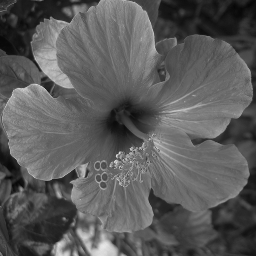
\includegraphics[width=.30\linewidth]{chapter-sampling/original.png}&
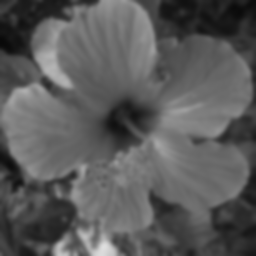
\includegraphics[width=.30\linewidth]{chapter-sampling/blurred.png}&
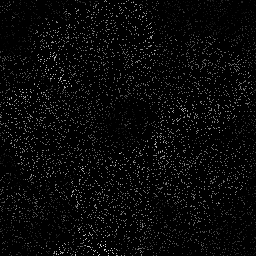
\includegraphics[width=.30\linewidth]{chapter-sampling/masked.png}\\
$f$&$\Phi f$ : flou&$\Phi f$ : masque
\end{tabular}
\caption{Deux opérateurs d'observation sans bruit appliqués à la même image de fleur : un flou gaussien et un masque conservant environ $10\%$ des pixels. Les valeurs manquantes sont affichées en noir.}\label{fig-exemple-ip}
\end{figure}

Plusieurs problèmes classiques entrent dans ce cadre :
\begin{itemize}
\item Débruitage : $\Phi=\mathrm{Id}$ et $P=Q$.
\item Déconvolution : $\Phi f=\phi\star f$, où le filtre $\phi$ décrit le flou et où les conditions au bord sont précisées.
\item Données manquantes : $\Phi$ sélectionne les coordonnées observées. On peut aussi conserver le tableau complet et utiliser le masque diagonal $\Phi=\operatorname{diag}(\mu_q)$, avec $\mu_q\in\{0,1\}$.
\item Tomographie : $\Phi$ modélise des intégrales de l'objet le long de droites, comme une transformée de Radon discrétisée.
\end{itemize}
Si $\Phi$ a un noyau non trivial, les seules mesures ne déterminent pas $f$. Même lorsqu'une matrice carrée $\Phi$ est inversible, ses petites valeurs singulières peuvent amplifier les erreurs dans $\Phi^{-1}y=f+\Phi^{-1}w$. La régularisation apporte une information supplémentaire pour sélectionner une reconstruction utile et stable.

\subsection{Régularisation parcimonieuse}
L'hypothèse $f\approx\Psi x$ avec peu de coefficients actifs conduit à
\begin{equation}\label{eq-pbm-l0}
 x^\star\in\arg\min_{\norm{x}_0\le M}\norm{y-\Phi\Psi x}_2^2,
 \qquad f^\star=\Psi x^\star.
\end{equation}
Pour le débruitage dans une base orthonormale, on obtient un seuillage dur des coefficients du \emph{signal observé $y$}. Il fournit le meilleur ajustement parcimonieux à $y$ pour le budget choisi ; il ne garantit pas, à lui seul, la plus petite erreur par rapport au signal propre inconnu $f$. Pour un opérateur d'acquisition général, $\Phi\Psi$ n'est pas orthogonal et la formule de seuillage ne résout plus le problème.

Les algorithmes gloutons et la relaxation convexe proposent deux façons d'aborder cette difficulté~\cite{MallatMP,2014-vaiter-ps-review}. Pour motiver la relaxation convexe, considérons
\[
 \norm{x}_\alpha^\alpha=\sum_{n=1}^N|x_n|^\alpha,\qquad \alpha>0.
\]
Pour chaque vecteur $x$ fixé, cette quantité tend vers $\norm{x}_0$ lorsque $\alpha\downarrow0$. Les ensembles $B_\alpha=\{x:\sum_n|x_n|^\alpha\le1\}$ sont contenus dans $[-1,1]^N$ et convergent, pour la distance de Hausdorff, vers
\[
 B_0=\{x\in[-1,1]^N:\norm{x}_0\le1\}.
\]
Cet ensemble limite est constitué de segments portés par les axes de coordonnées, y compris l'origine. L'ensemble $\{x:\norm{x}_0\le1\}$ sans restriction au cube contient, lui, les axes entiers et n'est pas borné.

\begin{figure}[htbp]\centering
\begin{tabular}{@{}c@{\hspace{2mm}}c@{\hspace{2mm}}c@{\hspace{2mm}}c@{\hspace{2mm}}c@{}}
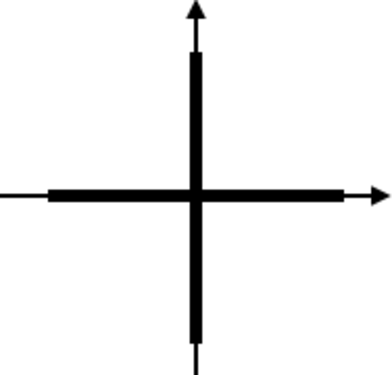
\includegraphics[width=.185\linewidth]{balls/l0}&
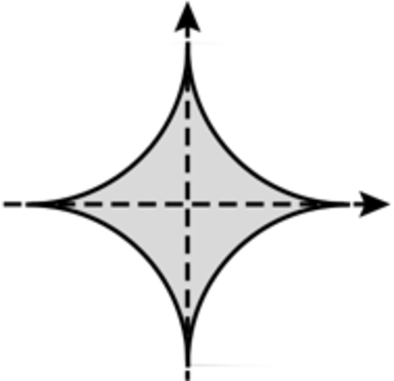
\includegraphics[width=.185\linewidth]{balls/l12}&
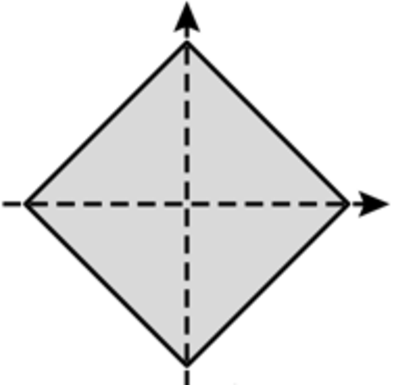
\includegraphics[width=.185\linewidth]{balls/l1}&
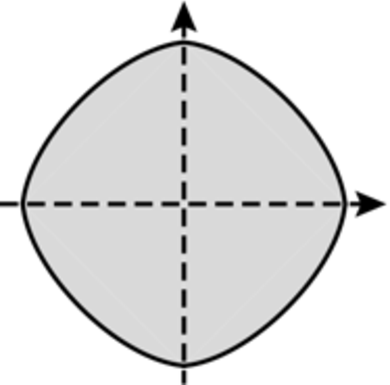
\includegraphics[width=.185\linewidth]{balls/l32}&
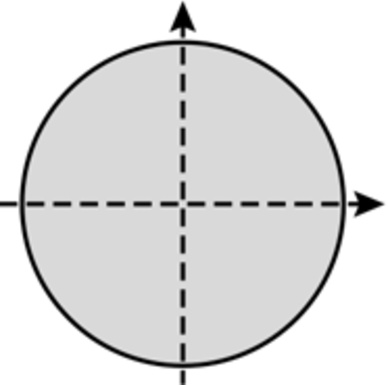
\includegraphics[width=.185\linewidth]{balls/l2}\\
$\alpha=0$&$\alpha=1/2$&$\alpha=1$&$\alpha=3/2$&$\alpha=2$
\end{tabular}
\caption{Les ensembles $B_\alpha$ en dimension deux. Le premier panneau représente l'ensemble limite borné $B_0$.}\label{fig-boules}
\end{figure}

Dans cette famille, $\norm{\cdot}_\alpha$ est une norme et $B_\alpha$ est convexe exactement lorsque $\alpha\ge1$. Le choix $\alpha=1$ associe la convexité à une géométrie qui favorise les coefficients nuls. On obtient ainsi le problème du Lasso sous contrainte
\begin{equation}\label{eq-pbm-l1}
 x^\star\in\arg\min_{\norm{x}_1\le\tau}\frac12\norm{Ax-y}_2^2,
 \qquad A=\Phi\Psi.
\end{equation}
Augmenter $\tau$ permet de mieux ajuster les mesures, mais peut aussi conduire à reproduire leurs erreurs. Ce paramètre se choisit en fonction du bruit, de l'opérateur et du modèle de signal. Faire tendre $\tau$ vers l'infini supprime la régularisation et laisse généralement plusieurs reconstructions possibles lorsque $P<N$.

Deux formulations proches sont utiles :
\begin{align}
 &\min_x\ \frac12\norm{Ax-y}_2^2+\lambda\norm{x}_1,
 &&\lambda>0,\label{eq-lasso-penalized}\\
 &\min_x\ \norm{x}_1\quad\text{sous la contrainte }\norm{Ax-y}_2\le\varepsilon,
 &&\varepsilon\ge0.\label{eq-bpdn}
\end{align}
La formulation pénalisée équilibre fidélité aux données et parcimonie. La seconde, appelée \emph{basis pursuit denoising}, est commode lorsqu'une borne d'erreur $\varepsilon$ est connue. Pour $\varepsilon=0$, elle devient le problème de \emph{basis pursuit}, $\min_{Ax=y}\norm{x}_1$. Ces formulations sont reliées par des multiplicateurs de Lagrange appropriés ; leurs paramètres ne sont pas des valeurs numériques interchangeables. Leurs premiers développements concernent notamment l'inversion sismique, la décomposition par \emph{basis pursuit} et le Lasso~\cite{santosa1986linear,chen1999atomi,tibshirani1996regre}.

\begin{figure}[htbp]\centering
\begin{tabular}{@{}c@{\hspace{3mm}}c@{\hspace{3mm}}c@{}}
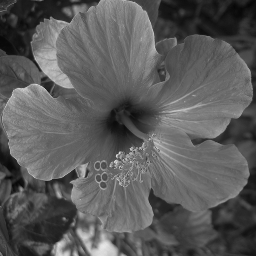
\includegraphics[width=.30\linewidth]{chapter-sampling/original.png}&
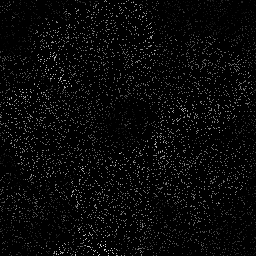
\includegraphics[width=.30\linewidth]{chapter-sampling/masked.png}&
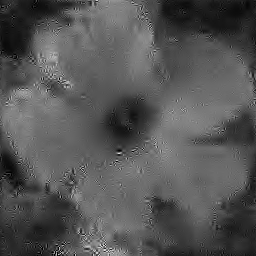
\includegraphics[width=.30\linewidth]{chapter-sampling/reconstructed.png}\\
$f$&$y$&$f^\star=\Psi x^\star$
\end{tabular}
\caption{Reconstruction à partir de 6\,554 pixels observés sur $256^2$, soit environ $10\%$. Le problème pénalisé~\eqref{eq-lasso-penalized} est résolu numériquement avec $\lambda=0{,}005$, des intensités dans $[0,1]$ et les mêmes ondelettes orthonormales qu'à la figure~\ref{fig-approx}. Les erreurs de texture restantes illustrent les limites du modèle.}\label{fig-inpainting}
\end{figure}

La convexité rend possible l'optimisation globale, mais la grande dimension et la non-différentiabilité de $\norm{x}_1$ demandent des algorithmes adaptés. Les méthodes proximales exploitent le seuillage doux explicite associé à cette pénalité~\cite{combettes2011proximal}. Un solveur numérique atteint une précision prescrite, plutôt qu'une solution réelle exacte après un petit nombre d'opérations garanti.

\subsection{Le rôle de la géométrie}
En dimension deux, la boule $\ell^1$ possède des sommets sur les axes de coordonnées. Un ensemble de niveau du terme d'attache aux données peut rencontrer la boule pour la première fois en l'un de ces sommets, ce qui produit un coefficient nul. Dans la même configuration, la boule ronde $\ell^2$ donne généralement deux coefficients non nuls (figure~\ref{fig-l1-vs-l2}). Cette géométrie explique une tendance, sans garantir le résultat pour tout opérateur et toute donnée : un contact le long d'une face peut donner plusieurs minimiseurs, et une solution $\ell^1$ n'est pas nécessairement assez parcimonieuse pour retrouver le signal recherché.

\begin{figure}[htbp]\centering
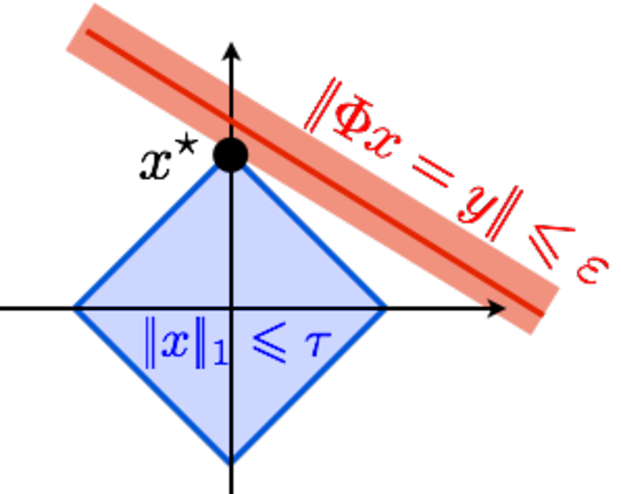
\includegraphics[width=.36\linewidth]{l1-vs-l2/l1}\hspace{8mm}
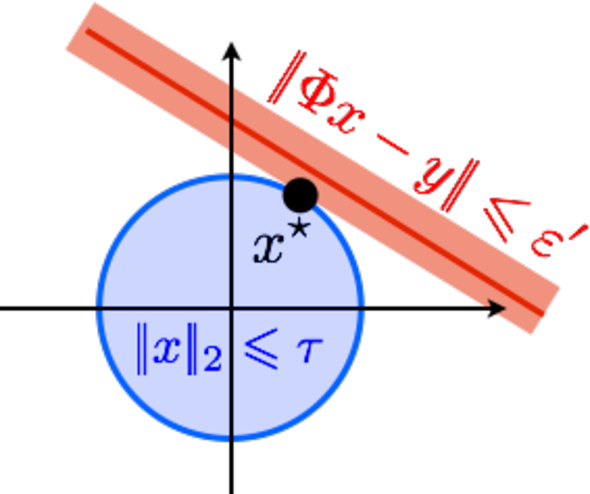
\includegraphics[width=.36\linewidth]{l1-vs-l2/l2}
\caption{Ajustement aux données sous une contrainte $\ell^1$ (à gauche) ou $\ell^2$ (à droite). À partir de $\varepsilon=0$, on élargit la bande $\{x:\norm{Ax-y}_2\le\varepsilon\}$ jusqu'à son premier contact avec la boule de contrainte. Le point de contact minimise le résidu sur cette boule.}\label{fig-l1-vs-l2}
\end{figure}

La reconstruction dépend de l'action de l'opérateur de mesure sur les vecteurs parcimonieux. Augmenter la dimension ambiante ne suffit pas à l'améliorer. Des conditions précises existent pour de nombreux opérateurs aléatoires et structurés ; la convolution et l'acquisition de Fourier demandent des hypothèses adaptées à leur géométrie~\cite{candes-towards2013,2015-duval-focm,AdcockBreaking,Chauffert14}.

\section{Acquisition comprimée}
\subsection{Mesurer des combinaisons de pixels}
Le codage par transformée commence par acquérir $Q$ échantillons, puis en conserve une représentation beaucoup plus petite. L'acquisition comprimée cherche à mesurer directement $P\ll Q$ combinaisons linéaires bien choisies et à reconstruire un signal parcimonieux, ou approximativement parcimonieux, dans une base connue.

La caméra à pixel unique développée à l'université Rice illustre cette idée~\cite{DuarteSinglePixel}. Une grille de $Q$ micromiroirs dirige certaines portions de la lumière vers un détecteur unique ; les autres miroirs les dirigent ailleurs. Pour chaque configuration $p$, le détecteur mesure la somme
\[
 y_p=\sum_{q=1}^Q\Phi_{p,q}\int_{c_q}\tilde f(s)\,\d s+w_p
     =\sum_{q=1}^Q\Phi_{p,q}f_q+w_p,
 \qquad \Phi_{p,q}\in\{0,1\}.
\]
Les miroirs n'enregistrent pas les pixels individuels. Changer leur configuration produit directement le vecteur $y\in\RR^P$. La scène doit rester suffisamment stable pendant ces mesures. Des configurations complémentaires, ou une mesure étalonnée de la lumière totale, permettent de convertir les mesures $0/1$ en mesures signées centrées.

\begin{figure}[htbp]\centering
\begin{tabular}{@{}c@{\hspace{2mm}}c@{\hspace{2mm}}c@{}}
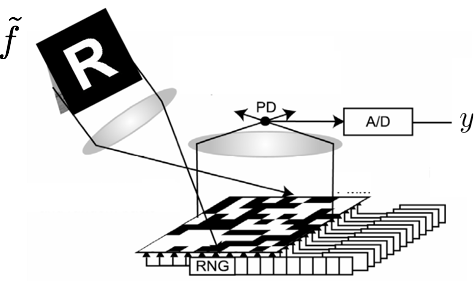
\includegraphics[width=.45\linewidth]{single-pixel/single-pixel-schema}&
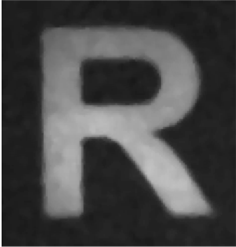
\includegraphics[width=.24\linewidth]{single-pixel/reconstruction-1}&
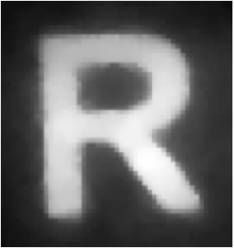
\includegraphics[width=.24\linewidth]{single-pixel/reconstruction-6}\\
Acquisition&$f$&$f^\star$
\end{tabular}
\caption{Acquisition à pixel unique et exemple de reconstruction original, repris des documents associés à~\cite{DuarteSinglePixel}. Le facteur annoncé de réduction du nombre de mesures est $Q/P=6$, donc $P/Q\approx1/6$.}\label{fig-single-pixel}
\end{figure}

\subsection{Une garantie de reconstruction}
Voici une forme classique de la garantie d'acquisition comprimée~\cite{candes2006stable,donoho2006compressed}. Supposons que $\Psi$ soit une base orthonormale de $\RR^N$, que $f=\Psi x_0$ et que $A=\Phi\Psi$ ait des entrées gaussiennes indépendantes, de moyenne nulle et de variance $1/P$. On peut, de façon équivalente, choisir $\Phi$ suivant cette loi gaussienne, qui est invariante par multiplication par une matrice orthogonale fixée.

Il existe des constantes universelles positives $C,c,C_0,C_1$ telles que, pour $1\le M\le N$ et
\begin{equation}\label{eq-cs-contrainte}
 P\ge C M\log(eN/M),
\end{equation}
avec une probabilité au moins égale à $1-2e^{-cP}$ sur le choix de $A$, la borne suivante soit vraie simultanément pour tous les $x_0$ et toutes les erreurs vérifiant $\norm{w}_2\le\varepsilon$. Toute solution $x^\star$ de~\eqref{eq-bpdn}, avec $y=Ax_0+w$, satisfait
\begin{equation}\label{eq-cs-error}
 \norm{x^\star-x_0}_2
 \le C_0\frac{\sigma_M(x_0)_1}{\sqrt M}+C_1\varepsilon,
 \qquad
 \sigma_M(x_0)_1=\min_{\norm{z}_0\le M}\norm{x_0-z}_1.
\end{equation}
Le logarithme de~\eqref{eq-cs-contrainte} est naturel ; changer sa base modifie seulement la constante. Le régime comprimé intéressant est celui où le nombre requis $P$ reste inférieur à $N$.

La quantité $\sigma_M(x_0)_1$ est la somme des amplitudes des coefficients éliminés après conservation des $M$ plus grands. Si $x_0$ est exactement $M$-parcimonieux et si l'on choisit $\varepsilon=0$ dans le problème sans bruit (donc $w=0$), les deux termes de~\eqref{eq-cs-error} s'annulent : le \emph{basis pursuit} retrouve exactement $x_0$. Pour les signaux approximativement parcimonieux et les mesures bruitées, ces termes séparent l'erreur d'approximation de l'erreur de mesure. L'orthonormalité donne la même erreur euclidienne sur le signal reconstruit : $\norm{\Psi x^\star-f}_2=\norm{x^\star-x_0}_2$.

Une démonstration de ce théorème passe par la propriété d'isométrie restreinte : $A$ préserve approximativement les longueurs euclidiennes des vecteurs portés par des ensembles suffisamment petits. Les matrices aléatoires vérifient cette propriété lorsque le nombre de mesures est de l'ordre indiqué dans~\eqref{eq-cs-contrainte}. Des modèles sous-gaussiens centrés appropriés admettent aussi des garanties, avec des constantes dépendant de leur loi. Pour une matrice brute à entrées $0/1$, il faut tenir compte du centrage et de la normalisation ; ce n'est pas le modèle gaussien énoncé ci-dessus.

Le théorème porte sur un nombre de mesures réelles, et non sur un nombre de bits. Leur précision, leur quantification et leur stockage restent à prendre en compte. L'algorithme de reconstruction doit connaître la matrice de mesure, par exemple grâce à une graine aléatoire partagée. Garder cette matrice secrète ne constitue pas, à lui seul, une garantie de sécurité cryptographique. De même, les économies de temps ou d'énergie dépendent du dispositif physique et du coût de reconstruction.

Les acquisitions structurées, notamment en imagerie par résonance magnétique, imposent des contraintes supplémentaires : on ne peut généralement pas choisir des mesures gaussiennes indépendantes arbitraires. Les trajectoires d'échantillonnage et les modèles de parcimonie doivent donc être étudiés ensemble~\cite{AdcockBreaking,Chauffert14}. Le principe directeur reste de concevoir conjointement l'acquisition et la reconstruction, en s'appuyant sur un modèle adapté aux données.

\paragraph*{Pour aller plus loin.}
Les liens entre approximation, problèmes inverses et optimisation dépassent la parcimonie. D'autres pénalités décrivent la régularité, le faible rang ou la structure géométrique. L'article de synthèse~\cite{2014-vaiter-ps-review} développe ces idées, et les Numerical Tours~\cite{2011-peyre-cise} proposent des expériences numériques.

\ifdefined\StandaloneChapter
\paragraph*{Remerciements.}
Je remercie Charles Dossal, Jalal Fadili, Samuel Vaiter, Stéphane Seuret et le rapporteur anonyme du texte original pour leur aide.
\fi
